\documentclass[conference]{IEEEtran}
\IEEEoverridecommandlockouts
% The preceding line is only needed to identify funding in the first footnote. If that is unneeded, please comment it out.
\usepackage{cite}
\usepackage{amsmath,amssymb,amsfonts}
\usepackage{graphicx}
\usepackage{textcomp}
\usepackage{url}
\usepackage{algorithm2e}
\usepackage{xcolor}
\usepackage{multirow}
\def\BibTeX{{\rm B\kern-.05em{\sc i\kern-.025em b}\kern-.08em
T\kern-.1667em\lower.7ex\hbox{E}\kern-.125emX}}
\begin{document}

% Custom commands:
\newcommand{\coo}{\ensuremath{\mathrm{CO_2}}}

% -----------------------------------
% -------------- TITLE --------------
\title{RoadAI - A Multi-agent Reinforcement Learning Approach to Reducing \coo{} Emissions at a Construction Site}
% -----------------------------------



% -----------------------------------
% ------------- AUTHORS -------------
% -----------------------------------
\author{
	\IEEEauthorblockN{Viktor Ringvold Hasle}
	\IEEEauthorblockA{\textit{Dept. of Informatics} \\
	\textit{University of Oslo}\\
	Oslo, Norway \\
	viktorrh@ifi.uio.no}
	\and
	\IEEEauthorblockN{Ada Hatland}
	\IEEEauthorblockA{\textit{Dept. of Informatics} \\
	\textit{University of Oslo}\\
	Oslo, Norway \\
	adaha@ifi.uio.no
	}
	\and
	\IEEEauthorblockN{Elias Lynum Ringkjøb}
	\IEEEauthorblockA{\textit{Dept. of Informatics} \\
	\textit{University of Oslo}\\
	Oslo, Norway \\
	eliaslr@ifi.uio.no
	}
	\and
	\\
	\IEEEauthorblockN{Tom Frode Hansen}
	\IEEEauthorblockA{\textit{NGI- Norges Geotekniske Institutt} \\
	Oslo, Norway \\
	tom.frode.hansen@ngi.no
	}
}

\maketitle


% -----------------------------------
% ------------ ABSTRACT -------------
% -----------------------------------
\begin{abstract}
\coo{} gas is one of the major contributors to greenhouse gases. Reducing greenhouse gases is an essential
task in reducing the environmental impacts of global warming. From extreme weather to the ruin of ecosystems
and mass extinctions, it is clear that global warming, caused by greenhouse gases, is a major existential issue.
In Norway, 1.5\% of the total \coo{} emissions come from construction machines. Given the total greenhouse gas
emissions adding up to almost 50 million metric tonnes of \coo{} equivalences, a reduction in emissions from
construction machines will lead to a significant reduction in the country's total emissions.

Although there have been studies conducted that use Reinforcement Learning techniques to reduce emissions by
optimizing routes and scheduling, our attempt in this paper is to extend this to the use of Multi-Agent
Reinforcement Learning techniques. The field of Multi-Agent Reinforcement Learning has gained more and more
applications recently, and has been used in various optimization problems.

This paper demonstrates implementations of Multi-Agent versions of two well-tested Reinforcement Learning
methods: Proximal Policy Optimization and Deep Q-Networks. It shows the promising results of how 
Multi-Agent Reinforcement Learning could be used to reduce \coo{} emissions, but it also highlights many ways in
which these methods can be improved.


% Should have 3-5 keywords.
Index Terms - Multi-Agent Reinforcement Learning (MARL), Emissions reduction. Road Construction.
\end{abstract}
  

% -----------------------------------
% - INTRODUCTION  -
% -----------------------------------
\section{Introduction}
Carbon dioxide (\coo{}) emission is one of the largest contributions to greenhouse gasses and global warming.
Reducing \coo{} emissions is an important step in preventing global warming and all of the negative
consequences associated with it. Norway's total greenhouse gas emissions were, according to Statistics
Norway, in 2022 48.9 million tonnes of \coo{} equivalences. \cite{SSB_2023}
1.5\% of these are emitted by construction machines. \cite{noraRoadAIReducing} The reduction of such
a significant part of the total emissions is a crucial task.

This project is based on the RoadAI competition held by Norwegian Artificial Intelligence Research
Consortium (NORA). \cite{noraRoadAIReducing} The objective in the RoadAI competition was to improve
sustainability at a road construction site using data driven methods. For this paper, we have taken the
task i an a somehwat different direction, and will present a method for using multi-agent Reinforcement
Learning (MARL) algorithms in order to reduce construction machine emissions.

% Green House Gas (GHG) emissions and the effects of global warming
% <TODO>

% RL for GHG reduction
In \cite{MORADI2022111882}, the goal was to use Reinforcement Learning (RL) for route optimization in
an attempt to reduce \coo{} emissions. The study used an implementation of three
different RL algorithms in order to optimize the ship's speed and direction: Deep Q-Network (DQN),
Deep Deterministic Policy Gradient (DDPG) and Proximal Policy Optimization (PPO). The study reported a
saving in fuel consumption of between approx. 1 and 6 percent, where DDPG demonstrates the best result,
and DQN yields the least improvement.

Another study, \cite{HUO2023106664}, showed promising results in reduction of greenhouse gas
emissions
from dump trucks' fuel consumption in a open-pit mining fleet. This model is a Q-learning RL algorithm
which aims to improve fleet productivity, and decreasing idle time, which in turn reduces the greenhouse
gas emissions. It does so by offering a real-time, reactive,  dispatching system, rather than a manual
fixed one. The RL model, trained on a simulated environment, takes into account traffic, queueing,
payload and maintenence requirements. As a result, the model showed an up to 30\% reduction in greenhouse
gases while having no impact on production levels.

% MARL
The field of Multi-agent Reinforcement Learning (MARL) is an emerging field in informatics. We see a wide
range of applications, such as robotics where it's been used to make joints in a single robot more
cooperative with others, \cite{Perrusquia_Yu_Li_2020} as well as using MARL in a system with multiple robots
to either compete or cooperate in order to get a task done. \cite{Wang2022}
Other usages of MARL is in railroad scheduling \cite{laurent2021flatland} and solving various games.
\cite{ellis2022smacv2}, \cite{yu2022surprising}

There is a diverse set of use cases for MARL. This paper will be presenting a way of implementing
MARL techniques seen in \cite{Perrusquia_Yu_Li_2020}, \cite{Wang2022}, \cite{laurent2021flatland},
\cite{ellis2022smacv2} and \cite{yu2022surprising} to expand upon the works done in emissions reduction
with single-agent RL \cite{HUO2023106664} and \cite{MORADI2022111882}.


% Environments
% <TODO>

% PPO / MAPPO
Proximal Policy Optimization (PPO) is an RL algorithm used mostly for single-agent reinforcement learning.
This is due to the fact that PPO is often considered less sample-effective than other off-policy algorithms
when it comes to MARL problems. In \cite{yu2022surprising}, however, they showed the effectiveness of the PPO
algorithm on multi-agent cooperative problems.

Several implementations of PPO for multi-agent problems have been shown tp yield good results in articles such
as \cite{ellis2022smacv2} and \cite{laurent2021flatland}.


% DQN / QMIX?
\cite{ellis2022smacv2} reported good results using the QMIX algorithm on the SMAC environment. QMIX is an
MARL algorithm based on Deep Q-Network (DQN). DQN is described in \cite{DBLP:journals/corr/MnihKSGAWR13} to
produce groundbreaking results in various gaming environments.


% Our work
The purpose of this paper is to highlight the use of MARL algorithms in order to reduce \coo{} emissions
from construction sites. This is done through reducing the distance driven by dump trucks at the site,
reducing idle time and optimal route finding in order to reduce acceleration due to topography. In this
paper, we will demonstrate an implementation of two different MARL algorithms:
(1) multi-agent PPO (MAPPO) and (2) multi-agent DQN. In addition to these algorithms, we have implemented a
custom environment based on \texttt{gymnasium}. \cite{Towers_Gymnasium}

Our work shows the potential of MARL algorithms to reduce emissions at construction sites using MARL
algorithms. The model is learning, however it is learning very slowly. This shows the potential of
the algorithms tested in this paper, but there is room for improvement.


% -----------------------------------
% ------------- METHODS -------------
% -----------------------------------
\section{Methodology}
The goal of the RoadAI project is to demonstrate an algorithm that could reduce emissions from road construction.
We are using MARL to train agents on a simulation of road construction and to demonstrate how it can be utilized to solve this problem.
Our methodology primarily focuses on the utilization of Multi-Agent Reinforcement Learning to tackle the problem of emissions in road construction. Given the complexity of the task, we adopted a step-by-step approach to ensure that the model is not only accurate but also efficient.


\subsection{Problem Formulation}
The first step in our methodology was to formulate the problem in the context of MARL. We defined each construction vehicle as an agent with its own set of actions, observations, and rewards. The joint action space consisted of moving, idling, loading, or unloading materials. Observations for each agent included the status of the road construction, the position of other agents, and the current load of materials. Rewards were also implemented to promote actions that lead to reduced emissions.



\subsection{Simulation Environment}
To train our agents, we developed a custom simulation environment using \texttt{gymnasium}. The environment replicates a typical road construction site, with details like topography and material locations. In this environment every object is represented as a particle in a grid.
The agents of the simulation, construction trucks are able to move cardinally in this grid with the goal of hauling construction materials from excavators to the unfinished road.
Every agent gets assigned a reward for each action they take with positive rewards for productive moves, and negative rewards for unproductive ones (idling, or unnecessary moving).

While simulating the trucks we collect the rewards which the reinforcement learning algorithms uses to train.
Using the average episodic rewards we can estimate the algorithms performance over the training, and compare them to each other.

\begin{figure}[!ht]
	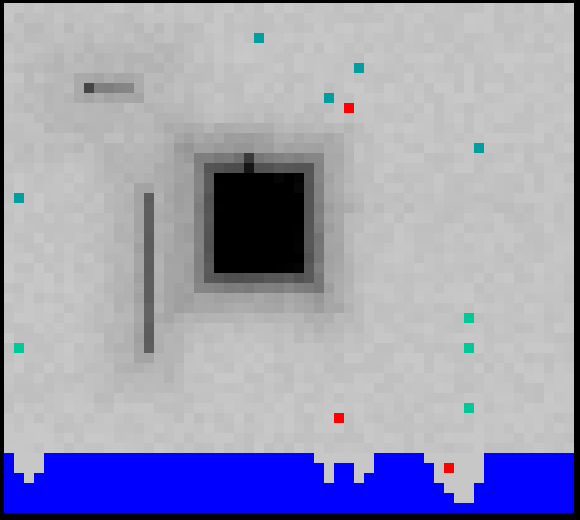
\includegraphics[width=\columnwidth]{graphs/example_env.png}
	\caption{Example randomly generated environment}
\end{figure}

While this environment is very simplified in contrast to real life, it is easy to randomly generate.


\subsection{Agent Architecture}
The agents (which are represented as the red pixels in Figue 1.) are designed in accordance to the gym api.
The action space is the discrete set $[0 \ldots 4]$ where $0$ is idling, and the remaining values equals the cardinal directions.
The observation space is defined as a \texttt{gymnasium Dict} with the following fields:
\begin{enumerate}
	\item \texttt{Filled}: whether the truck is loaded.
	\item \texttt{Pos}: the current position of the agent.
	\item \texttt{Adj}: a $5\times 5$ view of the closest tiles.
	\item \texttt{Target}: the position of the closest excavator
\end{enumerate}
Using a named dictionary for the observation space makes it easier to explain what the agents are actually observing in the environment.


\subsection{MAPPO}
We used the Stable-Baselines implementation of the PPO algorithm to train our agents.
PPO is an actor-critic method that is currently considered state of the art, and has
been shown to produce good results in similiar cooperative environments. % INSERT SITATION HERE
It implements clipping of the gradient to ensure we don't overshoot when climbing.
It is also stochastic by design where the policy $\pi_\theta$ chooses random actions
according to a certain heat which decreases over time.

Using PPO is a reasonable choice for this project as it's very sample efficient when learning, which
is important when getting training examples is a very time consuming project.
Even though we didnt manage to make use of real world examples to train, this might have been relevant
in the future if this project is expanded upon. It is shown later in this paper that DQN learns
faster than PPO in our specific project.

\begin{algorithm}[!ht]
  Initialize actor function $\pi$ with weigths $\theta$ \\
  Initialize critic function $V$ with weights $\phi$\\
  \For{$k = 0,1,2\ldots$}{
    Collect set of trajectories $D_k = \{\tau_i \}$ by running policy $\pi_k = \pi(\theta_k)$ \\
    Compute rewards-to-go $\hat{R}_t$\\
    Compute advantage emstimates $\hat{A}_t$ based on $V$\\
    Update the policy by maximizing: \\
    $ \sum_{\tau}^{D_k} \sum_{t}^T \ \min \left( \frac{\pi_\theta(a_t \mid s_t)}{\pi_{\theta k}(a_t \mid s_t)} A^{\pi_{\theta k}}(s_t, a_t), \mathbf{clip}(A^{\pi_{\theta k}}(s_t, a_t), \epsilon) \right) $ using gradient ascent\\
    Update the critic by regression via gradient descent:
    $ \sum_{\tau}^{D_k} \sum_{t = 0}^T \left( V_\phi (s_t) - \hat{R}_t\right)^2$
  }
\end{algorithm}


\subsection{Multi-agent DQN}
We first attempted to implement a version of DQN where the reward for an action is given as the average reward for
all the actions in that timestep. The issue with this is that it might reward a "bad" action and
punish a "good" action if the average reward that timestep was high or low respectively, it turns
out not treating it as a cooperative system but rather a system where every agent attempts to
maximise their own reward is significantly more efficient.

It's possible that with better hyperparameters or longer training time our multi agent
implementation of DQN might outperform the single agent implementation, but with the training
time and hyperparameters used we struggled to get positive rewards at all with this approach.

We ended up using the Stable-Baselines3 implementation of DQN, which may have affected the
difference in performance as well as the attempted multi agent DQN was based on the DQN tutorial
found at pytorch.org/tutorials/intermediate/reinforcement\_q\_learning.html. Having more than one
policy is important for research to make sure choice of policy doesn't heavily affect the outcome
of training. As is shown later in this paper, both of these methods performed quite similarly.

\begin{algorithm}[!ht]
  Initialize replaybuffer $D$ with capacity $N$\\
  Initialize action-value function $Q$ with weights $\theta$\\
  Initialize target-value function $\hat{Q}$ with weights $\hat{\theta}$\\
  \While{$t < N$}{
    Reset environment and set $o_t$\\
    \While{Episode is not finished}{
      With probablility $\epsilon$ select random action $a_t$\\
      Otherwise select $a_t = argmax_a \; Q(o_t, a ; \theta)$\\
      Execute $a_t$ in environment and get reward $r_t$ and $o_{t+1}$\\
      Store transition $\left( o_t, a_t, r_t, o_{t+1} \right)$ in $D$\\
      $t \gets t + 1$\\
    }
    Sample random minibatch $\bar{D}$ from $D$\\
    \For{$\left( o_j, a_j, r_j, o_{j+1} \right) \ \mathbf{in} \ \bar{D}$}{
      $y_j \gets r_j$ if epsisode terminates at $j$, $r_j + \gamma \hat{Q}(o_{t+1}, a';\hat{\theta})$ otherwise \\
      Gradient descent step $(y_j - Q(o_j, a_j; \theta))^2$ on $\theta$
    }
    Every C steps set $\hat{\theta} = \theta$\\

  }
\end{algorithm}


\subsection{Stable-Baselines}
While Stable-Baselines is not inherently compatible with multi-agent environments we found that if you
query the algorithm for each agent, and then return the observation for the next agent in line you could make it work in an MARL situation. This approach was suprisingly effective.
The custom training procedure would look something like this:

\begin{algorithm}[!ht]
	\For{$t = 0 \ \mathbf{to} \ N$}{
		$agent_{t} \gets env.agents[t\ \% \ M]$;\\
		$obs_t \gets agent_t.observe()$;\\
		$act_{t} \gets \theta(obs_{t})$; \\
		$env.step(act_t)$;\\
		$r_t \gets R(agent_t, act_t)$;\\
	}
\end{algorithm}

Where $N$ is maximum steps, $M$ is the number of agents, $R$ is the reward function, $\theta$ is the action function of the model action function.
Using this procedure allows us to iterate through every agent and enables Stable-baselines to be used in a Multi-agent setting.


\subsection{Training Procedure}
% Each algorithm was trained for 500 episiodes of a fixed length of 5000 steps. In total the training was
% 2.500.000 timesteps and took in total 2 hours on a NVIDIA GTX 3070 with 8gb of video ram.
\begin{tabular}{ |p{0.3\columnwidth}||p{0.5\columnwidth}|  }
  \hline
  \multicolumn{2}{|c|}{Training procedure parameters} \\
  \hline
  \hline
  Parameter         & Parameter value\\
  \hline
  Episodes          & 500\\
  \hline
  Steps per episode & 5,000\\
  \hline
  Total steps       & 2.5M\\
  \hline
  \hline
  Device used       & NVIDIA GTX 3070 w/ 8gb of video ram\\
  \hline
  Time              & Approx. 2 hours\\
  \hline
 \end{tabular}


\subsection{Hyperparameter Optimization}
We used the optuna library to hyperparameter optimize the PPO algorithm. Optuna uses a baynesian
search to find the best parameters for us. This way we could make sure that our results reach high
average rewards when combined with a fitting policy.

The following were the resulting hyperparameters after optimizing with Optuna:
\begin{tabular}{ |p{0.3\columnwidth}||p{0.5\columnwidth}|  }
  \hline
  \multicolumn{2}{|c|}{Hyperparameters post Optuna optimization} \\
  \hline
  \hline
  Parameter         & Parameter value\\
  \hline
  learning rate     & 0.001\\
  \hline
  clip range        & 0.20\\
  \hline
  gamma             & 0.95\\
  \hline
 \end{tabular}


% -----------------------------------
% ------------ REALITY GAP ----------
% -----------------------------------
\section{Reality Gap}



% -----------------------------------
% ------ RESULTS AND DISCUSSION -----
% -----------------------------------
\section{Results and Discussion}
Post-training, we evaluated our models based on following metrics:

\begin{enumerate}
	\item Mean episodic reward
	\item Total mass moved per episode
\end{enumerate}

The goal of these metrics was not only to see how our models performed throughout the training period, but also compare how the average rewards and mass hauled developed.

\begin{figure}[h!]
	%TODO ADD new image
	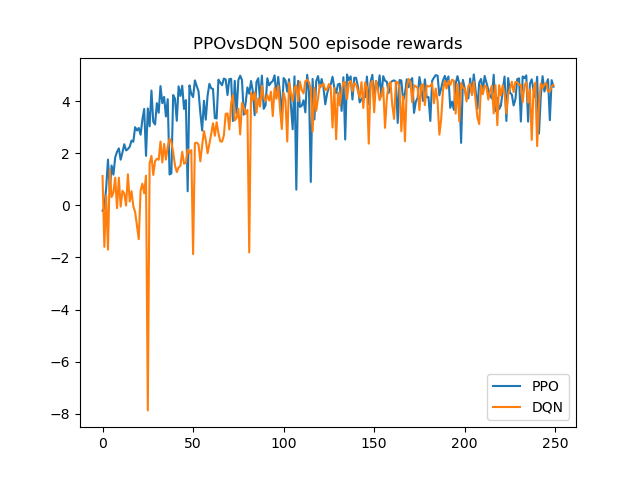
\includegraphics[width=\columnwidth]{graphs/PPOvsDQN250.png}
	\caption{Mean Episodic rewards}
\end{figure}
\begin{figure}[h!]
	%TODO ADD new image
	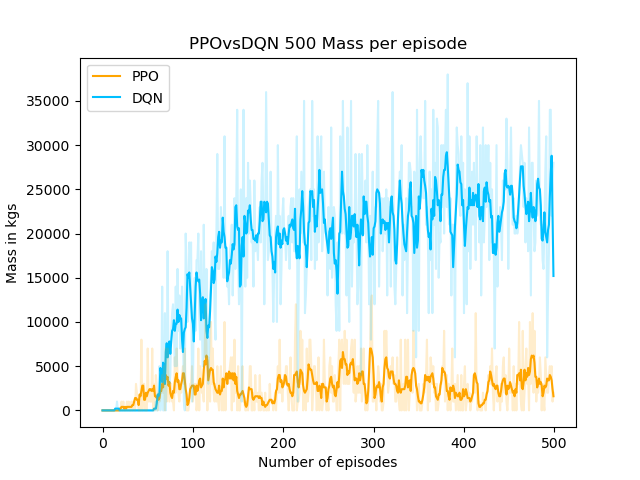
\includegraphics[width=\columnwidth]{graphs/PPOvsDQN500mass.png}
	\caption{Mass of construction materials moved per episode}
\end{figure}

As you could see from the graphs the algorithms performed quite similiarly.
Both algorithms managed to converge to what we could consider the reasonable optimum for the simulation
environment as we defined. Note that the amount of mass moved is increasing

Also noteworthy are the noticeable negative spikes, which indicate the points at which the agents got
stuck and were unable to perform their task. These spikes are more pronounced in the case of DQN,
suggesting that it might have a higher variance or instability during the learning process.

Overall, this test shows that both DQN and PPO can be effective algorithms for this type of reinforcement
learning task. However, the specific choice between the two might depend on other factors such as
computational resources, the complexity of the environment, and the desired speed and stability of
learning.


% \noindent


% -----------------------------------
% ---------- RELATED WORK -----------
% -----------------------------------
\section{Related works}
The \textit{SMACv2} \cite{ellis2022smacv2} research paper describes a new version of the StarCraft Multi-Agent
Challenge (SMAC), SMACv2. The SMAC testbed has been vital in the testing- and in turn improvement
of Multi-Agent ML algorithms. Given the updated version of SMAC, the team tested the performance og two
MARL- algorithms: (1) QMIX- a multi-agent implementation of DQN- and (2) MAPPO- Multi-Agent PPO. The
results yielded an up to 80\% win rate. The QMIX-algorithm generally performs better than that of MAPPO.
However, they note that MAPPO is still increasing its win rate towards the end of training, implying
that with further training, this algorithm could yield better results.

\textit{Flatlands-RL} \cite{laurent2021flatland} introduces an environment for testing MARL algorithms aimed at
solving the vehicle rescheduling problem (VRSP). They also test several RL and IL algorithms for
multiple agents with promising results for the MAPPO algorithm. This case shows the use of MARL in cooperative
multi-agent problems. However, the \textit{Flatlands-RL} paper is most concerned with solving the VRSP problem.

In the paper \textit{The Surprising Effectiveness of PPO in Cooperative, Multi-Agent Games}, \cite{yu2022surprising}
we see another case where a PPO-algorithm performs well in multi-agent problems.

We aim to evaluate MARL methods as a way to reduce \coo{} emissions at a construction site in this paper.
Seeing promising results for MAPPO in several related works, including \textit{Flatlands-RL} \cite{laurent2021flatland},
\textit{The Surprising Effectiveness of PPO [...]} \cite{yu2022surprising} and \textit{SMACv2} \cite{ellis2022smacv2}-
it is natural to choose this algorithm. In addition we will attempt a Multi-Agent implementation of DQN. Although the
overall goal of this paper isn't to compare MARL algorithms, this could yield some interresting results about the
usage of the two algorithms in this sort of problem.


% -----------------------------------
% ----------- CONCLUSION ------------
% -----------------------------------
\section{Conclusion}

The RoadAI competition goal was to reduce \coo{} emissions from the construction of roads.
The competition and dataset was certainly not created with a MARL solution in mind.
This papers goal was to lay the framwork for a possible MARL solution to the problem.
By training the agents on our custom environment we have shown that MARL algorithms can be used to solve
this  kind of problem.

There is however the big caveat that the reality gap between our environment and real life.
Real construction sites aren't perfectly square and trucks aren't pixels capable of turning in every
cardinal direction instantly. There is certainly more analysis needed on the cost-benefit tradeoff
between having a lightweight simple environment, or a more realistic and complex one.

Another big caveat is the lack of a proper baseline of comparasion to our solution.
Originally we had planned to compare our solution to the solutions of the others contestants in the
competion, but as far as we can tell no solution have been offically published, eventhough the competition
is concluded. Another approach would be to create the environment based on images from real-life
construction sites, and then compare the simulated trucks to the trucks in real life.

Keeping these caveats in mind, this paper still shows the promise of MARL algorithms to solve these kind of
problems where reinforcement learning doesn't traditionally come to mind.


% -----------------------------------
% ----------- FUTURE WORK -----------
% -----------------------------------
\section{Future work}

\subsection{Reward function}
	There are several potential improvements we could make to the reward function, that might alleviate the agents from performing some unwanted actions that currently occur.
	Firstly, sometimes an agent will get stuck north of a hill not realizing it can reach the holes it wants to fill by going around it and instead get stuck in a loop going up and down.
	Possible fixes are giving a penalty for going the wrong way or giving a possible reward for going sideways to encourage going around obstacles in cases where going the right way is impossible or not encouraged.
	Secondly multiple agents will sometimes get stuck trying to leave and fill holes among each other where all of them try to avoid colliding while also trying to go different ways.
	Their behaviour might be improved by giving them a penalty for being too close to one another or a reward for keeping proper distance, not just collision.

	\subsection{Environment and action space}
	Currently the environment we're using is a microgrid environment. This allows for moving up, down, right and left.
	While this is sufficient for a lot of states, in several cases we might want to go diagonally between two points as this means fewer steps, as well as a potentially shorter time between two holes are filled by one dump truck.
	Using a continuous environment instead with a continuous action space might cause the training time to increase but the asymptotic reward possible to reach would increase. The representation of the state could still be very similar to what it currently is, but the action space would significantly change.
	One possible implementation of this action space could instead of being a discrete set of directions be an angle and speed.
	As a consequence of this the reward function would also have to change, to not just encourage dump trucks to go for example 3000km/h to reach their goal in a single timestep, or not just give them a reward for getting closer to their goal, but how much distance is closed.
	The DQN approach would not be sufficient in this case because it is designed for discrete action spaces, PPO however is designed to both work for discrete and continuous action spaces.

\subsection{Environment and action space}
Currently the environment we're using is a microgrid environment. This allows for moving up, down, right and left.
While this is sufficient for a lot of states, in several cases we might want to go diagonally between two points as this means fewer steps, as well as a potentially shorter time between two holes are filled by one dump truck.
Using a continuous environment instead with a continuous action space might cause the training time to increase but the asymptotic reward possible to reach would increase. The representation of the state could still be very similar to what it currently is, but the action space would significantly change.
One possible implementation of this action space could instead of being a discrete set of directions be an angle and speed.
As a consequence of this the reward function would also have to change, to not just encourage dump trucks to go for example 3000km/h to reach their goal in a single timestep, or not just give them a reward for getting closer to their goal, but how much distance is closed.
The DQN approach would not be sufficient in this case because it is designed for discrete action spaces, PPO however is designed to both work for discrete and continuous action spaces.

\subsection{Environment creation}
Currently the environment is just created randomly with a certain set of features, excavators, agents and holes to be filled.
For our implementation to be viable in a real world setting it would be necessary to procuce environments from images of real construction sites, and it would be massively beneficial for the training set to be similarly constructed.
For this to be possible we would need a segmentation algorithm as well to find where all the important parts of the image are and either translate it into a microgrid like environment or simply use the image as well as the segmentation as the state and observation.
Along with making this change the environment and action space would likely have to be made continuous as discussed in the previous paragraph.
If the state is the image and not a transformation of the image into a microgrid or similar environment we would likely have to render each timestep as realistically as possible so it transfers nicely to the real world.
A better approach might be to transform it into a microgrid like environment and in the real world update it for example every 5 timesteps to the current state with a new image and new segmenting to make sure the real world doesn't deviate too far from what the environment looks like.
A way to implement this in training is to not make the environment entirely deterministic, and only update the environment to what it "actually" is every 5 timesteps.

% \begin{figure}[h!]
% 	%TODO ADD new image
% 	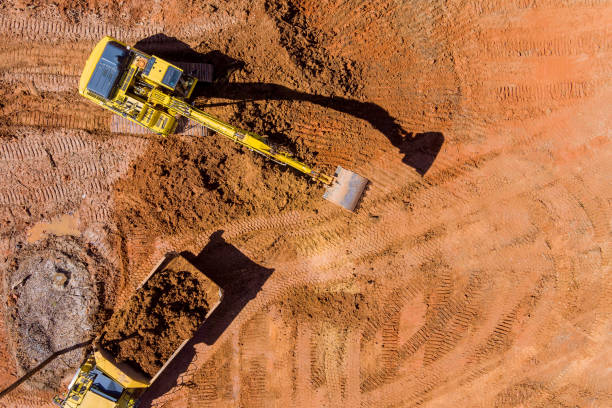
\includegraphics[width=\columnwidth]{graphs/construction_site.jpg}
% 	\caption{Example of what would need to be segmented}
% \end{figure}

\subsection{Agents}
Currently the excavators in our simulations are stationary, but in a real world scenario there isn't an infinite amount of mass where the excavators are stationed, so they would have to move every now and then, or possibly more often.
This could be done by moving the excavators to the closest depot whenever they empty the depot of gravel they're standing by, but a potential better solution is adding them to the pool of agents with their own actions, this will most likely increase training time but might very well increase performance over all.
Some minor changes should also likely be made to the dump truck agents to better resemble real world dump trucks.
Currently emptying and loading happens instantaneously, which is unrealistic. Its possible they require one or more timesteps to do, which would allow other agents to move in this time.
An excavator is also able to load more than a single dump truck at a time which is obviously impossible.

\subsection{Future work conclusion}
There are both small and big changes to be made. Due to limited time and resources we are not currently able to implement them, even though implementation of the smaller changes would not take a lot of time, the bigger issue is retraining the algorithm and measure performance before and after, if the change is performance based, but even in the case of realism based changes the training and graphs would have to be remade.


% % -----------------------------------
% % -------- Declaration of -----------
% % ------ competing interests --------
% % -----------------------------------
% \section{Declaration of competing interest}
% The authors declare no competing interests


% % -----------------------------------
% % ------- Data Availability ---------
% % -----------------------------------
% \section{Data availability}
% No datasets were used in this paper.
% % The RoadAI competition did, however, preset its participants with several relevant datasets, which we might have
% % used to evaluate our model given some more time.


% -----------------------------------
% -------- ACKNOWLEDGEMENTS ---------
% -----------------------------------
\section{Acknowledgements}
Thank you to the University of Oslo, Department of Informatics and the Robotics and
Intelligent Systems (ROBIN) research group for supporting this project. A special thanks goes to
Tom Frode Hansen from NGI - Norwegian Geotechnical Institute and the ROBIN group for guiding us through
this project.

Although the project is based on the RoadAI competition made by NORA, the idea of using multiple
agents with reinforcement learning was designed by Tom.



% -----------------------------------
% -------- ETHICS STATEMENT ---------
% -----------------------------------
% \newpage

% \appendices
\section{Ethics Statement}
In the course of our project on Multi-agent Reinforcement Learning, aimed at mitigating \coo{} emissions
from construction sites, we have conducted research that involves no experiments with human participants.
While this specific phase of our work does not directly raise concerns regarding wages or human
participation, it is essential to recognize that the technologies and methodologies we are developing
may eventually be applied in real-world settings where human interactions are integral. In such instances,
it becomes crucial to address ethical considerations associated with human safety and well-being.

We acknowledge that our current implementation serves as a simulation, and it is not as robust as a
real-world application would need to be. However, we are committed to exploring ways to ensure that the
agents, which are part of the system, incorporate safeguards to prevent harm to humans and machinery.
This commitment reflects our ethical responsibility to uphold the safety and welfare of individuals who
may interact with these agents in practical applications.

Moreover, our reinforcement learning framework includes a reward function that assigns a substantial
negative reward for agent collisions, with the intent of discouraging such incidents. The severity of
this negative feedback is designed to minimize the likelihood of agents crashing into one another. It
is important to note, though, that while our design minimizes such events, it does not guarantee their
complete avoidance.

% The dataset we have employed for this project, generated by Skanska Norge AS and provided by Norwegian
% Artificial Intelligence Research Consortium (NORA), does not contain any personally identifiable
% information. Although the dataset's availability has yet to be confirmed, it was shared with us by NORA
% following the conclusion of the RoadAI competition.

The primary objective of our project is to significantly reduce \coo{} emissions originating from
construction sites, potentially leading to substantial environmental and societal benefits.
Construction sites contribute 1.5\% of total Norwegian \coo{} emissions, making the reduction of
emissions in this sector a vital endeavour. Implementing our system across numerous construction sites
in Norway could result in a significant reduction in total \coo{} emissions, a crucial step toward a more
sustainable future.

In line with our commitment to ethical AI deployment, transparency and explainability need to be
addressed. It is imperative to ensure stakeholders can understand and trust the model's decisions.
Thus we have to make efforts to ensure that MARL algorithms are interpretable, allowing a comprehensive
understanding of factors influencing decisions.

Our research and project implementation do not support or enable any form of discrimination against
individuals or groups. Furthermore, they do not entail risks related to deception or harassment.
Our work is firmly rooted in legal activities and does not promote any restrictions on human rights.
Our ethical commitment is to conduct research and develop technologies that contribute to a greener,
more sustainable world without compromising the well-being of individuals or society as a whole.

% -----------------------------------
% ----------- REFERENCES ------------
% -----------------------------------
\newpage


\nocite{*}        % This includes all references that haven't been explicitly cited
\bibliography{citations.bib}
\bibliographystyle{plain}

\end{document}

% STRUCTURE:
% ----------

% Title - 1 sentence
%   (Your paper title should be specific, concise, and descriptive. Avoid using unnecessary words such as “new” or “novel”. Include keywords that will help a reader find your paper.)
%   Proposal: RoadAI - A Multi-agent Reinforcement Learning approach to reducing \coo{} emissions at a construction site

% Abstract - 4 sentences
%   (Provide a concise summary of the research conducted. Include the conclusions reached and the potential implications of those conclusions. Your abstract should also:
%   - consist of a single paragraph up to 250 words, with correct grammar and unambiguous terminology;
%   - be self-contained with no abbreviations, footnotes, references, or mathematical equations;
%   - highlight what is unique in your work;
%   - include 3-5 keywords or phrases that describe the research, with any abbreviations clearly defined,  to help readers find your paper.)

% Introduction - 0.5-1 pages
%   (Help the reader understand why your research is important and what it is contributing to the field.
%   - Start by giving the reader a brief overview of the current state of research in your subject area.
%   - Progress to more detailed information on the specific topic of your research.
%   - End with a description of the exact question or hypothesis that your paper will address.
%   Also state your motivation for doing your research and what it will contribute to the field.)

% Methods - 2.5-3 pages
%   (Formulate your research question. It should include:
%   - a detailed description of the question;
%   - the methods you used to address the question;
%   - the definitions of any relevant terminology;
%   - any equations that contributed to your work.
%   The methods section should be described in enough detail for someone to replicate your work.)

%   Description of research question

%   Environment

%   PPO

%   DQN

% Results and Discussion - 0.5-1 page
%   (Show the results that you achieved in your work and offer an interpretation of those results. Acknowledge any limitations of your work and avoid exaggerating the importance of the results.)

% Related Work - 1.5-2 pages
%   (Related work)

% Conclusion - 1 page
%   (Summarize your key findings. Include important conclusions that can be drawn and further implications for the field.)

%   Future work
%     (Discuss benefits or shortcomings of your work and suggest future areas for research.)

% Acknowledgements - ????
%   (You can recognize individuals who provided assistance with your work, but who do not meet the definition of authorship. The acknowledgments section is optional.)

% References